\documentclass[tikz,border=8pt]{standalone}
% Shared look for every TikZ diagram. Load with % Shared look for every TikZ diagram. Load with % Shared look for every TikZ diagram. Load with \input{../../tools/tikz-style.tex}
\usepackage[T1]{fontenc}
\usepackage{lmodern}
\renewcommand{\sfdefault}{lmr}  % diagrams use the same serif as the text
\usetikzlibrary{arrows.meta, positioning, shapes.geometric, calc, fit, backgrounds}
\definecolor{cblue}{HTML}{4C78A8}
\definecolor{corange}{HTML}{F58518}
\definecolor{cgreen}{HTML}{54A24B}
\definecolor{cred}{HTML}{E45756}
\definecolor{cpurple}{HTML}{B279A2}
\definecolor{cgrey}{HTML}{6B6B6B}
\tikzset{
  every picture/.style={font=\sffamily, line width=1.2pt},
  box/.style={draw=#1, fill=#1!12, rounded corners=4pt, align=center, inner sep=7pt, minimum height=1.1cm},
  box/.default=cgrey,
  arrow/.style={-{Stealth[length=3mm]}, draw=cgrey, line width=1.4pt},
  title/.style={font=\sffamily\bfseries\Large},
  note/.style={font=\sffamily\small, text=cgrey, align=center},
}
\AtBeginDocument{\hyphenpenalty=10000 \exhyphenpenalty=10000}

\usepackage[T1]{fontenc}
\usepackage{lmodern}
\renewcommand{\sfdefault}{lmr}  % diagrams use the same serif as the text
\usetikzlibrary{arrows.meta, positioning, shapes.geometric, calc, fit, backgrounds}
\definecolor{cblue}{HTML}{4C78A8}
\definecolor{corange}{HTML}{F58518}
\definecolor{cgreen}{HTML}{54A24B}
\definecolor{cred}{HTML}{E45756}
\definecolor{cpurple}{HTML}{B279A2}
\definecolor{cgrey}{HTML}{6B6B6B}
\tikzset{
  every picture/.style={font=\sffamily, line width=1.2pt},
  box/.style={draw=#1, fill=#1!12, rounded corners=4pt, align=center, inner sep=7pt, minimum height=1.1cm},
  box/.default=cgrey,
  arrow/.style={-{Stealth[length=3mm]}, draw=cgrey, line width=1.4pt},
  title/.style={font=\sffamily\bfseries\Large},
  note/.style={font=\sffamily\small, text=cgrey, align=center},
}
\AtBeginDocument{\hyphenpenalty=10000 \exhyphenpenalty=10000}

\usepackage[T1]{fontenc}
\usepackage{lmodern}
\renewcommand{\sfdefault}{lmr}  % diagrams use the same serif as the text
\usetikzlibrary{arrows.meta, positioning, shapes.geometric, calc, fit, backgrounds}
\definecolor{cblue}{HTML}{4C78A8}
\definecolor{corange}{HTML}{F58518}
\definecolor{cgreen}{HTML}{54A24B}
\definecolor{cred}{HTML}{E45756}
\definecolor{cpurple}{HTML}{B279A2}
\definecolor{cgrey}{HTML}{6B6B6B}
\tikzset{
  every picture/.style={font=\sffamily, line width=1.2pt},
  box/.style={draw=#1, fill=#1!12, rounded corners=4pt, align=center, inner sep=7pt, minimum height=1.1cm},
  box/.default=cgrey,
  arrow/.style={-{Stealth[length=3mm]}, draw=cgrey, line width=1.4pt},
  title/.style={font=\sffamily\bfseries\Large},
  note/.style={font=\sffamily\small, text=cgrey, align=center},
}
\AtBeginDocument{\hyphenpenalty=10000 \exhyphenpenalty=10000}

\begin{document}
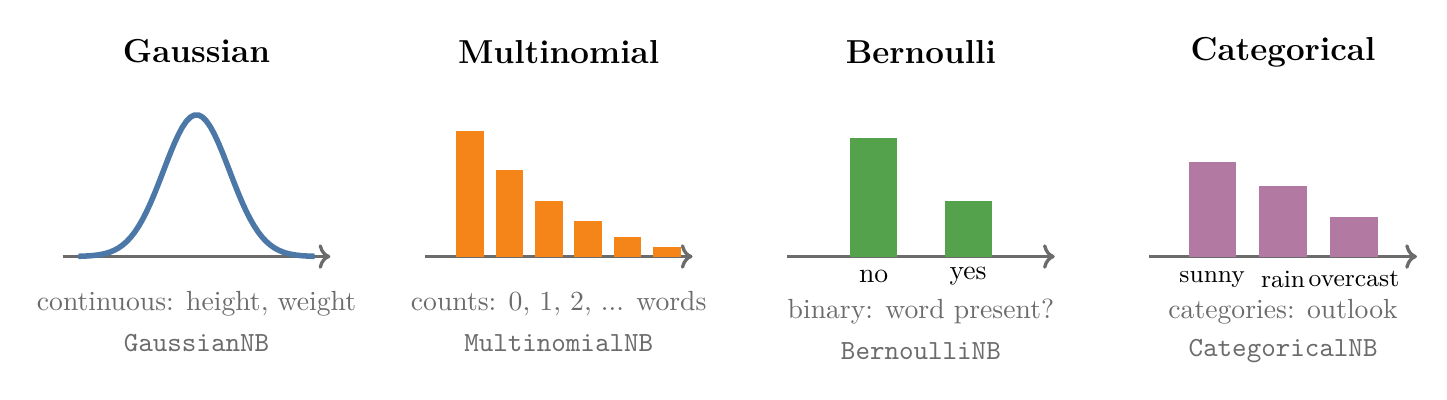
\begin{tikzpicture}[lab/.style={font=\sffamily\large\bfseries}, sub/.style={note, font=\sffamily}]
  % Gaussian: bell curve
  \begin{scope}[shift={(0,0)}]
    \draw[cgrey,->] (-0.2,0) -- (3.2,0);
    \draw[cblue, line width=2pt, domain=0:3, samples=60] plot (\x, {1.8*exp(-((\x-1.5)^2)/0.35)});
    \node[lab] at (1.5,2.6) {Gaussian};
    \node[sub] at (1.5,-0.6) {continuous: height, weight};
    \node[sub] at (1.5,-1.1) {\texttt{GaussianNB}};
  \end{scope}
  % Multinomial: counts
  \begin{scope}[shift={(4.6,0)}]
    \draw[cgrey,->] (-0.2,0) -- (3.2,0);
    \foreach \x/\h in {0.2/1.6, 0.7/1.1, 1.2/0.7, 1.7/0.45, 2.2/0.25, 2.7/0.12} \fill[corange] (\x,0) rectangle ++(0.35,\h);
    \node[lab] at (1.5,2.6) {Multinomial};
    \node[sub] at (1.5,-0.6) {counts: 0, 1, 2, ... words};
    \node[sub] at (1.5,-1.1) {\texttt{MultinomialNB}};
  \end{scope}
  % Bernoulli: yes/no
  \begin{scope}[shift={(9.2,0)}]
    \draw[cgrey,->] (-0.2,0) -- (3.2,0);
    \fill[cgreen] (0.6,0) rectangle ++(0.6,1.5); \fill[cgreen] (1.8,0) rectangle ++(0.6,0.7);
    \node[font=\sffamily] at (0.9,-0.25) {no}; \node[font=\sffamily] at (2.1,-0.25) {yes};
    \node[lab] at (1.5,2.6) {Bernoulli};
    \node[sub] at (1.5,-0.7) {binary: word present?};
    \node[sub] at (1.5,-1.2) {\texttt{BernoulliNB}};
  \end{scope}
  % Categorical
  \begin{scope}[shift={(13.8,0)}]
    \draw[cgrey,->] (-0.2,0) -- (3.2,0);
    \fill[cpurple] (0.3,0) rectangle ++(0.6,1.2); \fill[cpurple] (1.2,0) rectangle ++(0.6,0.9); \fill[cpurple] (2.1,0) rectangle ++(0.6,0.5);
    \node[font=\sffamily\small, anchor=north] at (0.6,-0.05) {sunny}; \node[font=\sffamily\small, anchor=north] at (1.5,-0.05) {rain}; \node[font=\sffamily\small, anchor=north] at (2.4,-0.05) {overcast};
    \node[lab] at (1.5,2.6) {Categorical};
    \node[sub] at (1.5,-0.7) {categories: outlook};
    \node[sub] at (1.5,-1.2) {\texttt{CategoricalNB}};
  \end{scope}
\end{tikzpicture}
\end{document}
